%!TEX root = edance.tex
%%%%%%%%%%%%%%%%
%  CHAPTER 13  %
%%%%%%%%%%%%%%%%
\chapter{Current Mirrors and Biasing}
\label{ch:ch13_mirrors_biasing}
\graphicspath{{./figures/figs_ch13_mirrors_biasing/}}
%%%%%%%%%%%%%%%%%%%%%%%%%%%%%%%%%%%%%%%%%%%%%%%%%%%%%%%%%%%%%%%%%%%%%%%%%%%%%%%%%%%%%%%%
%%%%%%%%%%%%%%%%%%%%%%%%%%%%%%%%%%%%%%%%%%%%%%%%%%%%%%%%%%%%%%%%%%%%%%%%%%%%%%%%%%%%%%%%
%                                   SECTION 13.1                                       %
%%%%%%%%%%%%%%%%%%%%%%%%%%%%%%%%%%%%%%%%%%%%%%%%%%%%%%%%%%%%%%%%%%%%%%%%%%%%%%%%%%%%%%%%
%%%%%%%%%%%%%%%%%%%%%%%%%%%%%%%%%%%%%%%%%%%%%%%%%%%%%%%%%%%%%%%%%%%%%%%%%%%%%%%%%%%%%%%%
\section{Chapter Preview}
This chapter begins by motivating the need for high load impedance in amplifiers.  Resistive loads have many drawbacks, including taking up a lot of physical space on an IC, and requiring a very large voltage headroom due to $IR$ voltage drops.  We introduce the basic current mirror, which can be used as a current source load in an amplifier with reduced headroom requirements.  Next we introduce an improved current source known as the cascode current source.  We discuss both NMOS and PMOS variants, which can be used to build current sources and current "sinks".  We conclude the chapter with an amplifier design example.
%%%%%%%%%%%%%%%%%%%%%%%%%%%%%%%%%%%%%%%%%%%%
%                 FIGURE                   %
%%%%%%%%%%%%%%%%%%%%%%%%%%%%%%%%%%%%%%%%%%%%
% \begin{figure}[H]
% \centering
% \includegraphics[scale=1.00]{null}
% \caption{null}
% \label{fig:ch13_intro}
% \end{figure}
%%%%%%%%%%%%%%%%%%%%%%%%%%%%%%%%%%%%%%%%%%%%
\newpage
%%%%%%%%%%%%%%%%%%%%%%%%%%%%%%%%%%%%%%%%%%%%
%                 FIGURE                   %
%%%%%%%%%%%%%%%%%%%%%%%%%%%%%%%%%%%%%%%%%%%%
\begin{figure}[t]
\centering
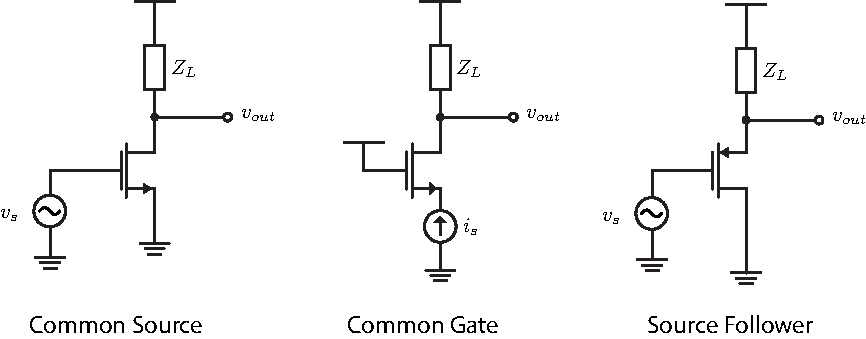
\includegraphics[width=.85\columnwidth]{0highZload.pdf}
\caption{High voltage gain amplifiers require a high load impedance $Z_L$.}
\label{fig:0highZload.pdf}
\end{figure}
%%%%%%%%%%%%%%%%%%%%%%%%%%%%%%%%%%%%%%%%%%%%
%                 FIGURE                   %
%%%%%%%%%%%%%%%%%%%%%%%%%%%%%%%%%%%%%%%%%%%%
\begin{figure}[H]
\centering
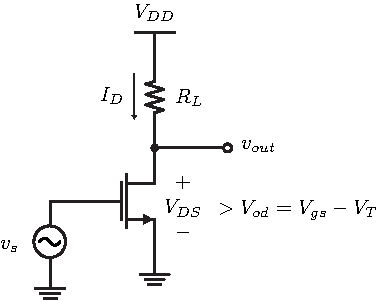
\includegraphics[scale=1]{1cs_headroom.pdf}
\caption{To maximize voltage gain, the transistor should operate in the saturation (or forward-active) region, which means $V_{DS} > V_{od}$ ($V_{CE} > V_{CE,sat}$), which places limits on how large we can make $R_L$ for a fixed bias current.}
\label{fig:1cs_headroom.pdf}
\end{figure}
%%%%%%%%%%%%%%%%%%%%%%%%%%%%%%%%%%%%%%%%%%%%%%%%%%%%%%%%%%%%%%%%%%%%%%%%%%%%%%%%%%%%%%%%
%%%%%%%%%%%%%%%%%%%%%%%%%%%%%%%%%%%%%%%%%%%%%%%%%%%%%%%%%%%%%%%%%%%%%%%%%%%%%%%%%%%%%%%%
%                                   SECTION 13.2                                       %
%%%%%%%%%%%%%%%%%%%%%%%%%%%%%%%%%%%%%%%%%%%%%%%%%%%%%%%%%%%%%%%%%%%%%%%%%%%%%%%%%%%%%%%%
%%%%%%%%%%%%%%%%%%%%%%%%%%%%%%%%%%%%%%%%%%%%%%%%%%%%%%%%%%%%%%%%%%%%%%%%%%%%%%%%%%%%%%%%
\section{High Load Impedance in Amplifiers}
%%%%%%%%%%%%%%%%%%%%%%%%%%%%%%%%%%%%%%%%%%%%
%             SUBSECTION 13.2.1            %
%%%%%%%%%%%%%%%%%%%%%%%%%%%%%%%%%%%%%%%%%%%%
\subsection{Load Impedance}
In each amplifier shown in \emph{Fig.~\ref{fig:0highZload.pdf}}, to maximize gain we should maximize the \textbf{load impedance}\index{Amplifier!load impedance} $Z_L$.  Can we just use an arbitrarily large load resistor?  In an IC process technology, resistors are realized either as diffusion regions or using polysilicon films.  The resistance per square is on the order of 100's to 1000's of ohms-per-square, which requires many squares to realize a large resistor, taking up a lot of area.  We are also limited in the minimum width of the resistor, because thinner resistors have limits on maximum current handling capability (due to self-heating).  Thinner resistors also experience wider variations from part to part, making the design gain more variable.  Next we will discuss the biggest limitation of all, which is simply the voltage drop across the resistors. 
%%%%%%%%%%%%%%%%%%%%%%%%%%%%%%%%%%%%%%%%%%%%
%             SUBSECTION 13.2.2            %
%%%%%%%%%%%%%%%%%%%%%%%%%%%%%%%%%%%%%%%%%%%%
\subsection{Headroom Limitations}
\index{Amplifier!headroom}
To keep the transistor in saturation requires $V_{DS} > V_{OD}$ (the over-drive voltage, $V_{GS} - V_T$).  For a fixed bias current, if we increase $R_L$, eventually we squash the transistor.  This means that it goes from the saturation region to the triode region, and the gain of the circuit is compromised.  This is illustrated in \emph{Fig.~\ref{fig:1cs_headroom.pdf}}.  One solution is to use a larger $V_{DD}$, but in practice this solution is hard to implement because each generation of IC technology has a voltage supply limit.  For example, today's nanoscale transistors can only tolerate $\sim 1\,V$ of voltage supply due to the thin oxides in the devices.  Even "thick oxide" devices, available for I/O\footnote{Iinput/output devices are used for driving external loads and receiving inputs from the outside of the chip.}, typically work at a maximum voltage of 2.5V or 3.3V (these voltage levels are standardized).
%%%%%%%%%%%%%%%%%%%%%%%%%%%%%%%%%%%%%%%%%%%%
%                 FIGURE                   %
%%%%%%%%%%%%%%%%%%%%%%%%%%%%%%%%%%%%%%%%%%%%
\begin{figure}[t]
\centering
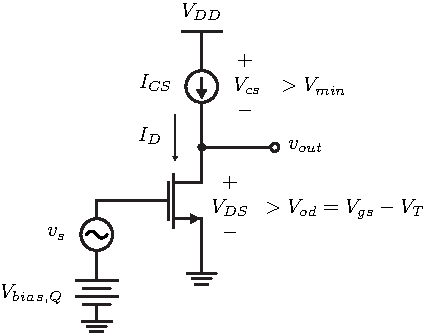
\includegraphics[width=.55\columnwidth]{2cs_current_mirror_load.pdf}\\
(a)\\
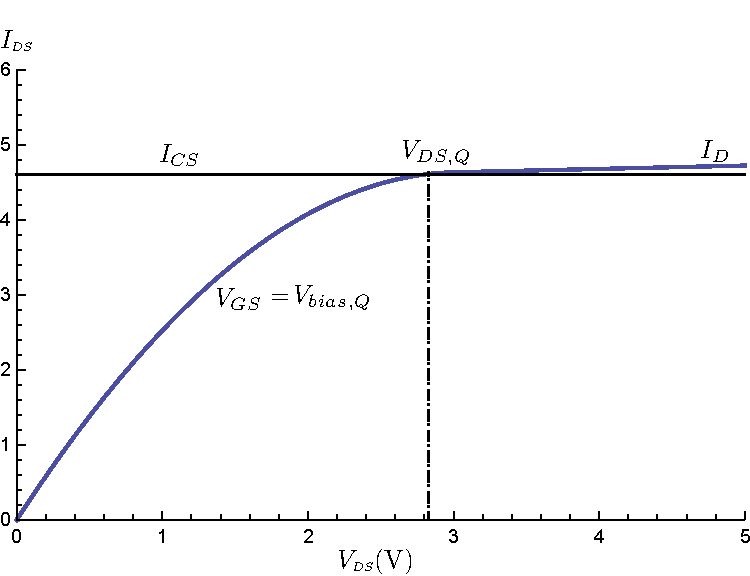
\includegraphics[width=.6\columnwidth]{mos_output_voltage.pdf}\\
(b)\\
\caption{(a) An ideal current source load results in the maximum gain for any bias current.  An ideal current source does not dictate the output voltage, just the current.  Note that $V_{bias,Q}$ determines the transistor operating point, which should match $I_{CS}$.  (b) The actual output voltage is determined by the transistor $I_{DS}$-$V_{DS}$ curve.}
\label{fig:2cs_current_mirror_load.pdf}
\end{figure}
%%%%%%%%%%%%%%%%%%%%%%%%%%%%%%%%%%%%%%%%%%%%
%             SUBSECTION 13.2.3            %
%%%%%%%%%%%%%%%%%%%%%%%%%%%%%%%%%%%%%%%%%%%%
\subsection{Achieving High Gain}
What if someone handed you a current source?  Then you could use it to bias the transistor, as shown in \emph{Fig.~\ref{fig:2cs_current_mirror_load.pdf}}.  Because an ideal current source has infinite output resistance, it would maximize the gain while supporting any value of $V_{DS}$.  Unfortunately, ideal current sources don't exist.  However, we could build one from a transistor with a fixed gate bias.  But how should we generate the correct bias voltage?  We will answer this question by first considering the wrong approach.
\newpage
%%%%%%%%%%%%%%%%%%%%%%%%%%%%%%%%%%%%%%%%%%%%
%                 FIGURE                   %
%%%%%%%%%%%%%%%%%%%%%%%%%%%%%%%%%%%%%%%%%%%%
\begin{figure}[t]
\centering
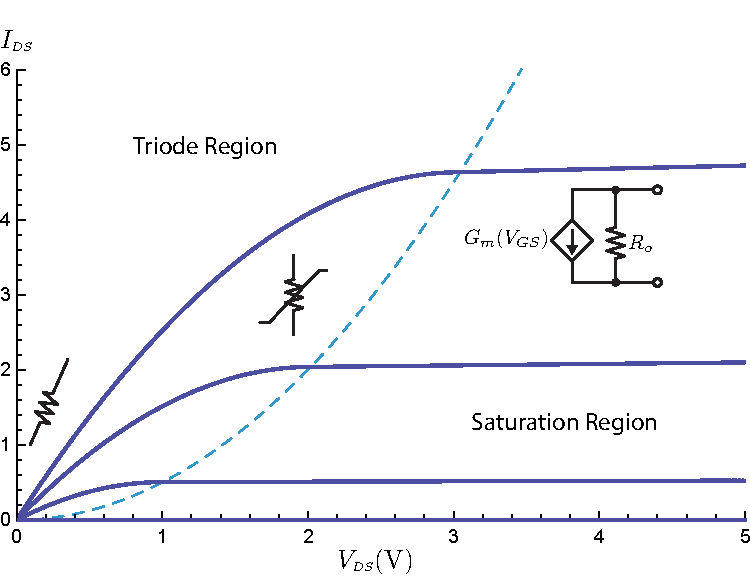
\includegraphics[width=.85\columnwidth]{mos_building_block.pdf}
\caption{An MOS transistor in the saturation region, or a BJT in the forward active region, has nearly constant current as a function of $V_{DS}$, making it a suitable proxy for an ideal current source if the output voltage does not go too low (or high for a PMOS transistor).  The gate voltage (base voltage) must be held constant at the appropriate bias voltage.}
\label{fig:mos_building_block.pdf}
\end{figure}
%%%%%%%%%%%%%%%%%%%%%%%%%%%%%%%%%%%%%%%%%%%%
%             SUBSECTION 13.2.4            %
%%%%%%%%%%%%%%%%%%%%%%%%%%%%%%%%%%%%%%%%%%%%
\subsection{Transistor Current Source}
A transistor biased in saturation with a constant $V_{GS}$ is effectively a decent current source, as shown in the $I$-$V$ curve in \emph{Fig.~\ref{fig:mos_building_block.pdf}}.  Even though the transistor is a dependent current source, the main source of dependence is the gate voltage, which we would like to hold constant.  The other dependence is the output resistance, which is much smaller, and results in non-zero slope in the $I$-$V$ curve. 
%%%%%%%%%%%%%%%%%%%%%%%%%%%%%%%%%%%%%%%%%%%%
%             SUBSECTION 13.2.5            %
%%%%%%%%%%%%%%%%%%%%%%%%%%%%%%%%%%%%%%%%%%%%
\subsection{Transistor Process / Temperature Variations}
If we simply fix the $V_{GS}$ value to realize a specific current, we are designing a current source that will have a very unpredictable output current.  For example, if the temperature varies, the threshold voltage changes, and so will the current.  Also, if we fix the gate bias value based on a model, then in real applications we will find that every transistor is a bit different from the model due to natural statistical variations (in doping levels and geometry, especially for small transistors).  So the output current will be a random variable with a large variance.  To keep the variance low we should use another strategy.

A good strategy is to observe that while two arbitrary transistors are not well matched, two transistors sitting right next to each other, or better yet two "inter-digitated transistors" (how this is done will be explained in \emph{Sec.~\ref{sec:interdigitate}}), will behave very similarly.  So the strategy should be to use one transistor to generate the $V_{GS}$ for the other.
\newpage
%%%%%%%%%%%%%%%%%%%%%%%%%%%%%%%%%%%%%%%%%%%%
%                 FIGURE                   %
%%%%%%%%%%%%%%%%%%%%%%%%%%%%%%%%%%%%%%%%%%%%
\begin{figure}[t]
\centering
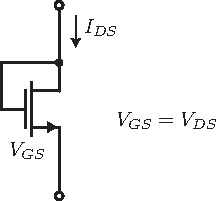
\includegraphics[scale=1.25]{3mos_diode.pdf}\\
(a)\\[0.25cm]
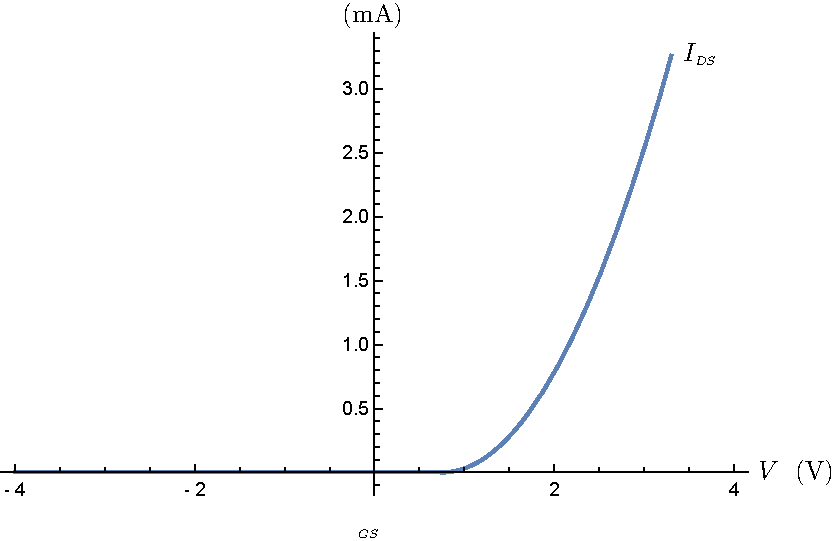
\includegraphics[width=.7\columnwidth]{ivrect.pdf}\\
(b)
\caption{(a) An MOS transistor with gate-drain shorted is known as a "diode connected" transistor.  It behaves as a non-linear unidirectional conductor, similar to a diode.  (b) The $I_{DS}$-$V_{GS}$ of a MOS diode is "rectifying" in that it only allows current to flow in one direction.}
\label{fig:3mos_diode.pdf}
\end{figure}
%%%%%%%%%%%%%%%%%%%%%%%%%%%%%%%%%%%%%%%%%%%%%%%%%%%%%%%%%%%%%%%%%%%%%%%%%%%%%%%%%%%%%%%%
%%%%%%%%%%%%%%%%%%%%%%%%%%%%%%%%%%%%%%%%%%%%%%%%%%%%%%%%%%%%%%%%%%%%%%%%%%%%%%%%%%%%%%%%
%                                   SECTION 13.3                                       %
%%%%%%%%%%%%%%%%%%%%%%%%%%%%%%%%%%%%%%%%%%%%%%%%%%%%%%%%%%%%%%%%%%%%%%%%%%%%%%%%%%%%%%%%
%%%%%%%%%%%%%%%%%%%%%%%%%%%%%%%%%%%%%%%%%%%%%%%%%%%%%%%%%%%%%%%%%%%%%%%%%%%%%%%%%%%%%%%%
\section{The Basic Current Mirror}
%%%%%%%%%%%%%%%%%%%%%%%%%%%%%%%%%%%%%%%%%%%%
%             SUBSECTION 13.3.1            %
%%%%%%%%%%%%%%%%%%%%%%%%%%%%%%%%%%%%%%%%%%%%
\subsection{Diode Connected Device}
The \textbf{diode connected MOS transistor}\index{MOSFET!types!diode connected}, shown in \emph{Fig.~\ref{fig:3mos_diode.pdf}}, is a two-terminal device.  It is never in the triode region, because of the gate-drain connection.  Since $V_{DS} = V_{GS}$, as long as $V_{GS}$ is over the threshold voltage, then the drain-source voltage is a threshold voltage away from saturation, since $V_{DS} = V_{GS} = V_{D,sat} + V_T$.  As we sweep $V_{GS}$ and observe the drain-source current, the transistor goes from "off" state (below threshold) to the "on" state.  It is called a diode because of the rectifying action of the the $I$-$V$ relation. Current can pass in one direction, but not the other, similar to a $PN$-junction diode.  The curve is not exponential, though, since the MOS device $I$-$V$ relation is quadratic.  If we pass a known current into a diode, the $V_{GS}$ value will be well-defined and equal to the value needed to generate the current. It is like an inverse function, that takes a current and generates the correct $V_{GS}$:
    \begin{equation*}
        V_{GS} = V_T + \sqrt{\frac{2\,I_{DS}}{\frac{W}{L} \mu C_{ox}}} = V_T + V_{OD}
    \end{equation*}
If the current injected into the device is very low, $V_{OD}$ will be low and the diode $V_{GS}$ will be approximately $V_T$.  In general for any current, the $V_{GS}$ generated can be used to bias a second transistor into the same current.
\newpage
%%%%%%%%%%%%%%%%%%%%%%%%%%%%%%%%%%%%%%%%%%%%
%             SUBSECTION 13.3.2            %
%%%%%%%%%%%%%%%%%%%%%%%%%%%%%%%%%%%%%%%%%%%%
\subsection{Diode Connected -- Small-Signal Model}
We can derive the small-signal model\index{Small-signal!model} by shorting out the gate-drain capacitor in the hybrid-$\pi$ model, shown in \emph{Fig.~\ref{fig:4mos_diode_ss.pdf}}.  Note that a $g_m$ generator with its controlling terminals connected to the $g_m$ is more simply a conductor.  From the perspective of the driving terminal, the MOS diode is just a conductance.
\vspace{1cm}
%%%%%%%%%%%%%%%%%%%%%%%%%%%%%%%%%%%%%%%%%%%%
%                 FIGURE                   %
%%%%%%%%%%%%%%%%%%%%%%%%%%%%%%%%%%%%%%%%%%%%
\begin{figure}[H]
\centering
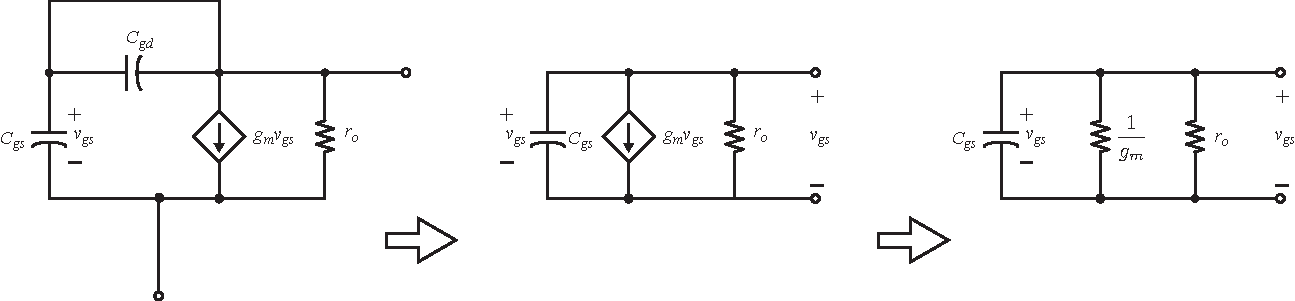
\includegraphics[scale=1.4]{4mos_diode_ss.pdf}
\caption{The small-signal model of a diode connected MOS transistor.  Notice that the model is simply a conductance when the gate-drain are shorted, as shown on the bottom.}
\label{fig:4mos_diode_ss.pdf}
\end{figure}
%%%%%%%%%%%%%%%%%%%%%%%%%%%%%%%%%%%%%%%%%%%%
\newpage
%%%%%%%%%%%%%%%%%%%%%%%%%%%%%%%%%%%%%%%%%%%%
%             SUBSECTION 13.3.3            %
%%%%%%%%%%%%%%%%%%%%%%%%%%%%%%%%%%%%%%%%%%%%
\subsection{The Integrated "Current Mirror"}
With the MOS diode as a voltage reference, we can build a \textbf{"current mirror"}\index{Current mirror}, shown in \emph{Fig.~\ref{fig:mirror_105}a}.  Since $M1$ and $M2$ have the same $V_{GS}$, as long as M2 is in saturation, they will carry approximately the same current.  If we neglect CLM ($\lambda = 0$), then the drain currents would be equal. Since $\lambda$ is small, the currents will nearly mirror one another even if $V_{out}$ is not equal to $V_{gs1}$. We say that the current $I_{in}$ is mirrored into $I_{out}$. Notice that the mirror works for small and large signals!

It is important to note that the diode side of the current is low impedance, due to the diode connection, as shown in \emph{Fig.~\ref{fig:mirror_105}b}.  On the other hand, from the drain of M2 the circuit presents a high impedance, thereby behaving like a current source.
\vspace{1cm}
%%%%%%%%%%%%%%%%%%%%%%%%%%%%%%%%%%%%%%%%%%%%
%                 FIGURE                   %
%%%%%%%%%%%%%%%%%%%%%%%%%%%%%%%%%%%%%%%%%%%%
\begin{figure}[H]
\centering
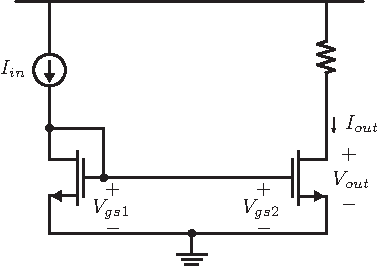
\includegraphics[scale=1.5]{5mirror_105.pdf}\\
(a)\\[1cm]
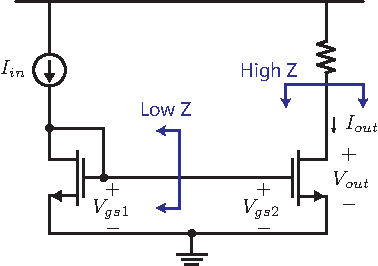
\includegraphics[scale=1.5]{5bmirror_105.pdf}\\
(b)
\caption{(a) An NMOS current mirror has an output current $I_{out}$ that is a "mirror copy" of $I_{in}$.  (b) The mirror has low impedance on the "diode" side and high impedance at the output.}
\label{fig:mirror_105}
\end{figure}
%%%%%%%%%%%%%%%%%%%%%%%%%%%%%%%%%%%%%%%%%%%%
\newpage
%%%%%%%%%%%%%%%%%%%%%%%%%%%%%%%%%%%%%%%%%%%%
%             SUBSECTION 13.3.4            %
%%%%%%%%%%%%%%%%%%%%%%%%%%%%%%%%%%%%%%%%%%%%
\subsection{Current Mirror with Multiplication Ratio} \label{sec:interdigitate}
As illustrated in \emph{Fig.~\ref{fig:mirror_amp}}, with some minor modifications, we can generate a mirror that \textbf{scales the input current up or down}\index{Current mirror!scaling}. The input and output currents are related as follows:
    \begin{equation}
        I_{IN} = k\left(\frac{W_1}{L_1}\right){(V_{GS_1} - V_T)}^2
    \end{equation}
    \begin{equation}
        I_{OUT} = k\left(\frac{W_2}{L_2}\right){(V_{GS_2} - V_T)}^2
    \end{equation}
The circuit connections forces the two transistors to operate at the same $V_{GS}$.  Assuming that they have the same threshold voltage (which is a good assumption if the transistors are nearby and laid-out together):
    \begin{equation}
        V_{GS1} = V_{GS2}
    \end{equation}
Which allows us to write:
    \begin{equation}
        I_{OUT} = k\left(\frac{W_2}{L_2}\right){(V_{GS_2} - V_T)}^2
        = I_{IN}\left(\frac{W_2/L_2}{W_1/L_1}\right) = N \cdot I_{IN}
    \end{equation}
In practice we prefer not to scale $L$, but rather the transistor widths $W$ to achieve the desired \textbf{scaling ratio}\index{Current mirror!scaling ratio} $N$ (unless $N$ is very large, then a combination of the both $L$ and $W$ will be scaled).  This is because the transistor threshold voltage and other parameters will vary with $L$, and it is best to match the two mirror transistors as much as possible, so they should have the same channel length.  In fact, the most accurate mirror is realized by inter-digitating two transistors, effectively connecting multiple unit transistors in parallel (see \emph{Fig.~\ref{fig:mirror_amp_n_copies}}), or better yet using multiple "fingers" in the layout of the transistors (see \emph{Fig.~\ref{fig:mirror_layout}}):
    \begin{align}
        \Aboxed{I_{OUT} &=  I_{IN}\left(\frac{W_2}{W_1}\right)
        = I_{IN}\left(\frac{N_2\cdot W_U}{N_1\cdot W_U}\right) = N \cdot I_{IN}}
        &\textit{Current mirror with scaling ratio}
        \label{eq:current_mirror_scaling}
    \end{align}
In \emph{Eq.~\ref{eq:current_mirror_scaling}}, $W_U$ is the unit transistor width.
\vspace{0.5cm}
%%%%%%%%%%%%%%%%%%%%%%%%%%%%%%%%%%%%%%%%%%%%
%                 FIGURE                   %
%%%%%%%%%%%%%%%%%%%%%%%%%%%%%%%%%%%%%%%%%%%%
\begin{figure}[H]
\centering
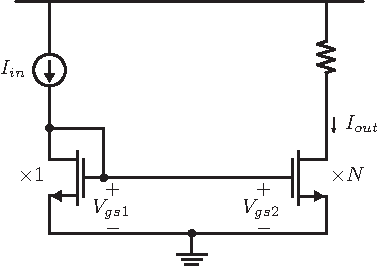
\includegraphics[scale=1.5]{6mirror_105_amp.pdf}
\caption{A current mirror can be configured to scale the input current by scaling the transistor dimensions $W/L$.}
\label{fig:mirror_amp}
\end{figure}
%%%%%%%%%%%%%%%%%%%%%%%%%%%%%%%%%%%%%%%%%%%%
\newpage
%%%%%%%%%%%%%%%%%%%%%%%%%%%%%%%%%%%%%%%%%%%%
%                 FIGURE                   %
%%%%%%%%%%%%%%%%%%%%%%%%%%%%%%%%%%%%%%%%%%%%
\begin{figure}[t]
\centering
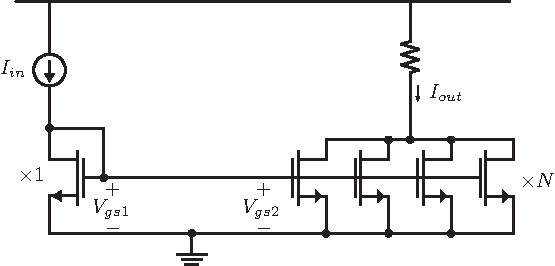
\includegraphics[scale=1.5]{6mirror_105_amp_Ncopies.pdf}
\caption{It is preferable to scale the input of a current mirror by scaling the transistor count, using parallel devices to realize a larger $W$.}
\label{fig:mirror_amp_n_copies}
\end{figure}
%%%%%%%%%%%%%%%%%%%%%%%%%%%%%%%%%%%%%%%%%%%%
%                 FIGURE                   %
%%%%%%%%%%%%%%%%%%%%%%%%%%%%%%%%%%%%%%%%%%%%
\begin{figure}[H]
\centering
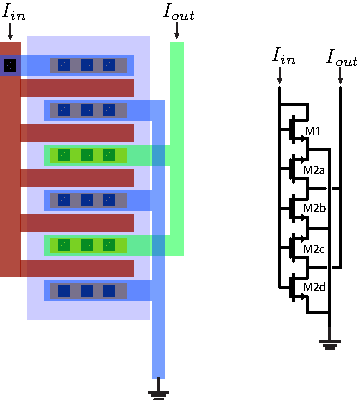
\includegraphics[width=.8\columnwidth]{mirror_layout.pdf} 
\caption{The layout of a 4:1 mirror using five unit elements. Note that transistors are abutted and source/drain junctions are shared to maximize matching between the gates, save area and minimize parasitics.  The input transistor is diode connected and the output transistor is split into four fingers.}
\label{fig:mirror_layout}
\end{figure}
%%%%%%%%%%%%%%%%%%%%%%%%%%%%%%%%%%%%%%%%%%%%
\newpage
%%%%%%%%%%%%%%%%%%%%%%%%%%%%%%%%%%%%%%%%%%%%
%                 FIGURE                   %
%%%%%%%%%%%%%%%%%%%%%%%%%%%%%%%%%%%%%%%%%%%%
\begin{figure}[t]
\centering
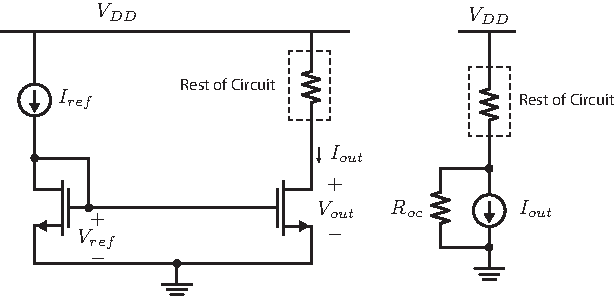
\includegraphics[scale=1.4]{7mirror_current_source.pdf}
\caption{From the perspective of the "rest of the circuit" shown, the current mirror appears like an ideal current source with output impedance $R_{oc}$.}
\label{fig:7mirror_current_source.pdf}
\end{figure}
%%%%%%%%%%%%%%%%%%%%%%%%%%%%%%%%%%%%%%%%%%%%
%                 FIGURE                   %
%%%%%%%%%%%%%%%%%%%%%%%%%%%%%%%%%%%%%%%%%%%%
\begin{figure}[H]
\centering
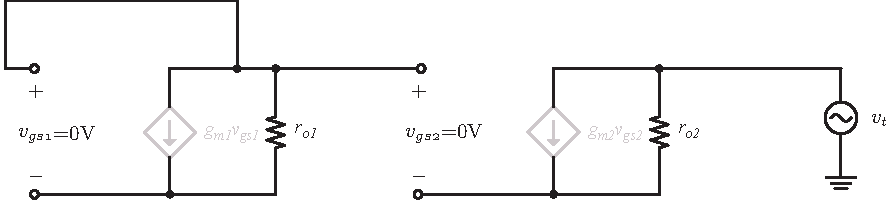
\includegraphics[scale=0.95]{8mirror_small_signal.pdf}
\caption{Current mirror small-signal model.  Transconductors are open-circuit (off) since the controlling voltages are zero.}
\label{fig:mirror_small_signal}
\end{figure}
%%%%%%%%%%%%%%%%%%%%%%%%%%%%%%%%%%%%%%%%%%%%
%             SUBSECTION 13.3.5            %
%%%%%%%%%%%%%%%%%%%%%%%%%%%%%%%%%%%%%%%%%%%%
\subsection{Current Mirror as Current Source}
As shown in \emph{Fig.~\ref{fig:7mirror_current_source.pdf}}, a current mirror acts like a current source to the rest of the circuit as long as the transistor $M2$ remains in saturation, where it has high output resistance.  Of course, there is a slight problem in that we need another voltage reference $I_{ref}$ to make this work.  The idea is that we generate one very accurate current reference using techniques that we will discuss in Section~\ref{sec:Ireference}, and this current reference can be mirrored around to various parts of the circuit using mirrors.  
%%%%%%%%%%%%%%%%%%%%%%%%%%%%%%%%%%%%%%%%%%%%
%             SUBSECTION 13.3.6            %
%%%%%%%%%%%%%%%%%%%%%%%%%%%%%%%%%%%%%%%%%%%%
\subsection{Small-Signal Resistance of Current Source}
The output impedance seen by the load can be calculated using the small-signal model\index{Small-signal!model} shown in \emph{Fig.~\ref{fig:mirror_small_signal}}.  Use a test generator $v_t$, and find the current draw from the source.  Note that $M1$ is not driven by a source, because $I_{ref}$ is DC, which means that it is an open circuit in the small-signal model.  Thus, without a source, $M1$ is effectively driven with zero $v_{gs}$ and has no output, pulling the $v_{gs}$ of both transistors to ground.  Then $M2$'s dependent $g_m$ is zero, and the only current draw is from $r_{o,2}$.
\newpage
%%%%%%%%%%%%%%%%%%%%%%%%%%%%%%%%%%%%%%%%%%%%
%                 FIGURE                   %
%%%%%%%%%%%%%%%%%%%%%%%%%%%%%%%%%%%%%%%%%%%%
\begin{figure}[t]
\centering
\begin{tabular}{c c}
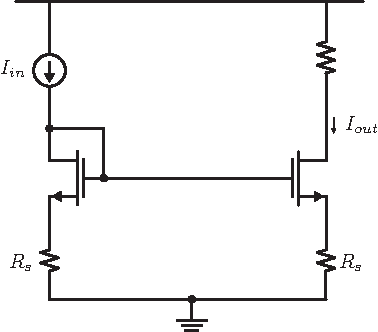
\includegraphics[scale=.85]{9mirror_Rs.pdf} & 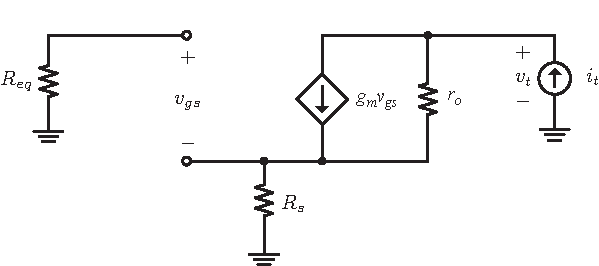
\includegraphics[scale=.85]{10mirrror_Rs_ss.pdf}\\
(a) & (b)
\end{tabular}
\caption{(a) Adding resistors in the source of a current mirror can be used to boost the output impedance at the cost of reducing the voltage headroom.  Note that the output impedance is boosted by a factor $g_m R_s$, rather than the additive factor of $R_s$, which would be true if the resistor were placed on the drain side.  (b) Small-signal model of improved output impedance mirror utilizing source resistance $R_s$.}
\label{fig:mirror_Rs}
\end{figure}
%%%%%%%%%%%%%%%%%%%%%%%%%%%%%%%%%%%%%%%%%%%%%%%%%%%%%%%%%%%%%%%%%%%%%%%%%%%%%%%%%%%%%%%%
%%%%%%%%%%%%%%%%%%%%%%%%%%%%%%%%%%%%%%%%%%%%%%%%%%%%%%%%%%%%%%%%%%%%%%%%%%%%%%%%%%%%%%%%
%                                   SECTION 13.4                                       %
%%%%%%%%%%%%%%%%%%%%%%%%%%%%%%%%%%%%%%%%%%%%%%%%%%%%%%%%%%%%%%%%%%%%%%%%%%%%%%%%%%%%%%%%
%%%%%%%%%%%%%%%%%%%%%%%%%%%%%%%%%%%%%%%%%%%%%%%%%%%%%%%%%%%%%%%%%%%%%%%%%%%%%%%%%%%%%%%%
\section{Improved Current Source:  The Cascode Mirror}
%%%%%%%%%%%%%%%%%%%%%%%%%%%%%%%%%%%%%%%%%%%%
%             SUBSECTION 13.4.1            %
%%%%%%%%%%%%%%%%%%%%%%%%%%%%%%%%%%%%%%%%%%%%
\subsection{Improved Current Sources}
The goal is to increase $R_{out}$ of the basic current mirror.  To get a hint about how to proceed, let's look at typical \textit{amplifier} output resistance results to see topologies that boost resistance.  The output impedance of the \textit{common gate} stage is boosted by placing a resistor in the source of the amplifier.  Likewise, the same is true of a \textit{common source} amplifier with \textbf{source degeneration}\index{Source degeneration}.  The same approach can be used to boost the output impedance of a mirror, as shown in \emph{Fig.~\ref{fig:mirror_Rs}a}.
%%%%%%%%%%%%%%%%%%%%%%%%%%%%%%%%%%%%%%%%%%%%
%             SUBSECTION 13.4.2            %
%%%%%%%%%%%%%%%%%%%%%%%%%%%%%%%%%%%%%%%%%%%%
\subsection{Effect of Source Degeneration}
Let's analyze the small-signal model of the mirror with $R_S$, as shown in \emph{Fig.~\ref{fig:mirror_Rs}b}.  We focus on the output side, or transistor $M2$, and model the input side as a Thévenin equivalent\index{Thévenin equivalent} resistance, $R_{eq}$, because there are no sources on the left side.  We inject a test current $i_t$ and measure the voltage developed across $i_t$:
    \begin{equation}
        v_t = (i_t - g_m\,v_{gs})r_o + v_{R_S}
    \end{equation}
First, note that the current $i_t$ flows through $R_S$ as it returns through the source.  This implies that the voltage across $R_S$ is given by:
    \begin{equation}
        v_{R_S} = i_t\,R_S
    \end{equation}
The key observation is that the current flowing in $R_S$ generates a gate-source voltage on the transistor, $v_{gs} = -v_{R_S}$.  This in turn creates a current through $g_m$:
    \begin{align}
        v_t &= \big(i_t - g_m\,(-v_{R_S})\big)r_o + v_{R_S}\\[0.25cm]
        &= (i_t + g_m\,R_S\,i_t)r_o + i_t\,R_S
    \end{align}
Collecting terms, we find that the output impedance is given by:
    \begin{equation}
        R_o = \frac{v_t}{i_t} = \left(1 + g_m\,R_S\right)r_o
    \end{equation}
\newpage
%%%%%%%%%%%%%%%%%%%%%%%%%%%%%%%%%%%%%%%%%%%%
%                 FIGURE                   %
%%%%%%%%%%%%%%%%%%%%%%%%%%%%%%%%%%%%%%%%%%%%
\begin{figure}[t]
\centering
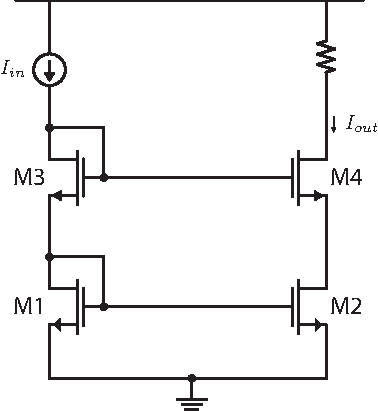
\includegraphics[scale=1]{12mirror_cascode.pdf}
\caption{An improved "cascode" or stacked current mirror.}
\label{fig:mirror_cascode}
\end{figure}
\noindent
%%%%%%%%%%%%%%%%%%%%%%%%%%%%%%%%%%%%%%%%%%%%
The output impedance is boosted by a factor of $(1 + g_m\,R_S)$, compared to a simple mirror.  How would you scale the output current?  If we use the same approach as before, we need to ensure that we scale the resistance as well:
    \begin{equation}
        I_{IN} = k \left(\frac{W_1}{L_1}\right){(V_G - V_S - V_T)}^2
    \end{equation}
where,
    \begin{equation}
        V_S = I_{IN}\,R_S
    \end{equation}
To keep $V_S$ the same, if $I_{OUT}$ is $N$ times larger, then $R_S$ should be $N$ times smaller.
%%%%%%%%%%%%%%%%%%%%%%%%%%%%%%%%%%%%%%%%%%%%
%             SUBSECTION 13.4.3            %
%%%%%%%%%%%%%%%%%%%%%%%%%%%%%%%%%%%%%%%%%%%%
\subsection{Cascode (or Stacked) Current Source}
The stacked current mirror, commonly known as the \textbf{cascode current mirror}\index{Amplifier!types!cascode current mirror}, is shown in \emph{Fig.~\ref{fig:mirror_cascode}}.  Notice that $V_{GS_2}$ is held constant like a normal mirror, but now $V_{DS_2}$ is also held  approximately constant by $M3/M4$.  This makes the output current variation much smaller than a single transistor. 

We can easily compute the boost in output impedance by noting that $R_S = r_{o_1}$ as far as transistor M4 is concerned: 
    \begin{equation}
        R_o \approx \left(1 + g_{m_2}\,R_S\right)r_{o_2} = \left(1 + g_{m_2}\;r_{o_1}\right)r_{o_2}
    \end{equation}
Which is approximately $g_m\,r_o$ times larger than a simple mirror:
    \begin{equation}
        R_o \approx g_{m_1}\,r_{o_1}\,r_{o_2} \gg r_o
    \end{equation}
%%%%%%%%%%%%%%%%%%%%%%%%%%%%%%%%%%%%%%%%%%%%
%             SUBSECTION 13.4.4            %
%%%%%%%%%%%%%%%%%%%%%%%%%%%%%%%%%%%%%%%%%%%%
\subsection{Drawback of Cascode Current Source}
Like all good things, there is a catch.  The minimum output voltage to keep all transistors in saturation increases, as shown in \emph{Fig.~\ref{fig:mirrors_vmin}}.  For a basic current mirror, we can go all the way down to $V_{OD}$ and keep $M2$ in saturation.  When we introduce $R_S$, we have to account for the extra $I_{OUT}\,R_S$ voltage drop.  With a cascode, the minimum voltage to keep $M4$ in saturation is given by noting that the source of $M4$ is biased by $M3$:
    \begin{equation}
        V_{S_4} = V_{G_4} - V_{GS_4}
        \label{eq:cascodesource}
    \end{equation}
%%%%%%%%%%%%%%%%%%%%%%%%%%%%%%%%%%%%%%%%%%%%
%                 FIGURE                   %
%%%%%%%%%%%%%%%%%%%%%%%%%%%%%%%%%%%%%%%%%%%%
\begin{figure}[H]
\centering
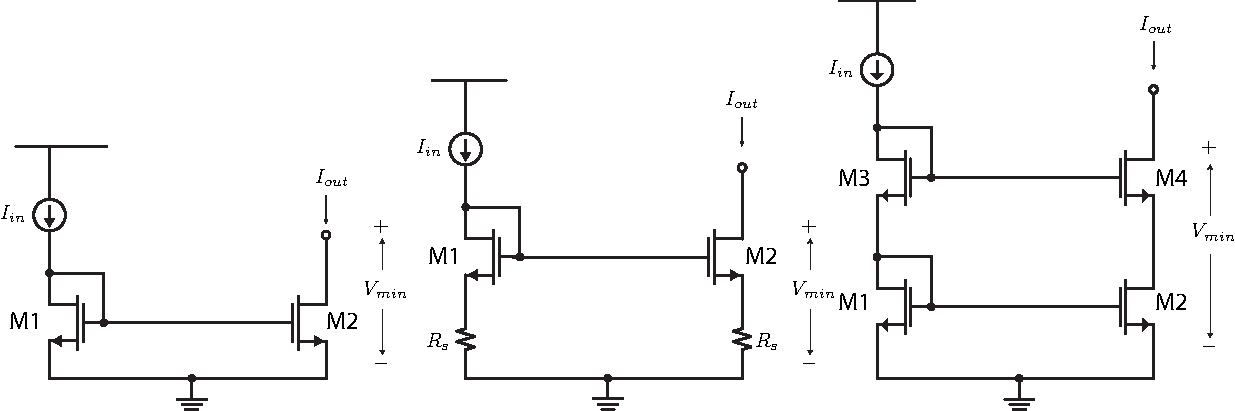
\includegraphics[width=\columnwidth]{mirrors_vmin}
\caption{Comparison of the reduction in the output swing of current mirrors as we improve the output impedance.}
\label{fig:mirrors_vmin}
\end{figure}
%%%%%%%%%%%%%%%%%%%%%%%%%%%%%%%%%%%%%%%%%%%%
The gate of transistor $M4$ is basically the $V_{GS}$ of $M1$ and $M3$:
    \begin{equation}
        V_{G_4} = V_{GS_1} + V_{GS_3} = 2\,V_T + 2\,V_{OV}
        \label{eq:cascodevgs}
    \end{equation}
To arrive at the RHS of \emph{Eq.~\ref{eq:cascodevgs}}, we assume that all devices have the same $V_T$ and size, so that the overdrive voltages are equal.  Since the $V_{GS_4} = V_T + V_{OD}$, we can write \emph{Eq.~\ref{eq:cascodesource}}:
    \begin{equation}
        V_{S_4} = V_{G_4} - V_{GS_4}   = 2\,V_T + 2\,V_{OD} - (V_T + V_{OD}) = V_T + V_{OD}
    \end{equation}
Now the minimum $V_{DS_4} = V_{OD}$ implies that the cascode mirror has a \textbf{minimum operating voltage}\index{Amplifier!cascode!minimum operating voltage} of:
    \begin{align}
        \Aboxed{V_{min} &= V_T + 2\,V_{OD}} &\textit{Cascode minimum operating voltage}
        \label{eq:cascode_min_voltage}
    \end{align}
This can be quite a large voltage penalty compared to a simple mirror, but an easy solution is to bias the gate of $M4$ with $V_T + 2 V_{OD}$ using a separate transistor, shown in \emph{Fig.~\ref{fig:cascode_hiswing}}.  The transistor overdrive voltage is twice as large by scaling the device down by $4\times$.  In a more advanced analog integrated circuits course you will learn about other ways to realize the \textbf{"high swing" cascode}\index{Amplifier!high swing cascode}.
%%%%%%%%%%%%%%%%%%%%%%%%%%%%%%%%%%%%%%%%%%%%
%                 FIGURE                   %
%%%%%%%%%%%%%%%%%%%%%%%%%%%%%%%%%%%%%%%%%%%%
\begin{figure}[H]
\centering
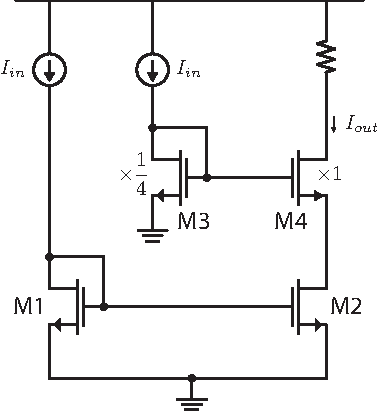
\includegraphics[scale=1]{mirror_cascode_hiswing.pdf}
\caption{To maximize the swing of a cascode mirror, the gate of the top "cascode" transistor $M4$ should be biased at $V_T + 2\,V_{OD}$ to place $M2$ at the edge of saturation.}
\label{fig:cascode_hiswing}
\end{figure}
%%%%%%%%%%%%%%%%%%%%%%%%%%%%%%%%%%%%%%%%%%%%
\newpage
%%%%%%%%%%%%%%%%%%%%%%%%%%%%%%%%%%%%%%%%%%%%
%                 FIGURE                   %
%%%%%%%%%%%%%%%%%%%%%%%%%%%%%%%%%%%%%%%%%%%%
\begin{figure}[t]
\centering
\begin{tabular}{cc}
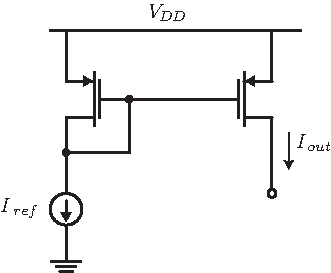
\includegraphics[scale=1.05]{18mirror_pmos.pdf} &
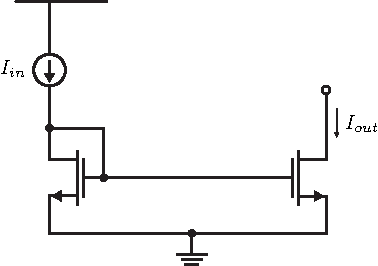
\includegraphics[scale=1.05]{nmos_source_mirror}\\ 
(a) & (b)\\
\end{tabular}
\caption{(a) A PMOS current source can "source" a current from supply.  (b) In contrast, an NMOS current can only "sink" a current to ground.}
\label{fig:mirror_pmos}
\end{figure}
%%%%%%%%%%%%%%%%%%%%%%%%%%%%%%%%%%%%%%%%%%%%
%                 FIGURE                   %
%%%%%%%%%%%%%%%%%%%%%%%%%%%%%%%%%%%%%%%%%%%%
\begin{figure}[H]
\centering
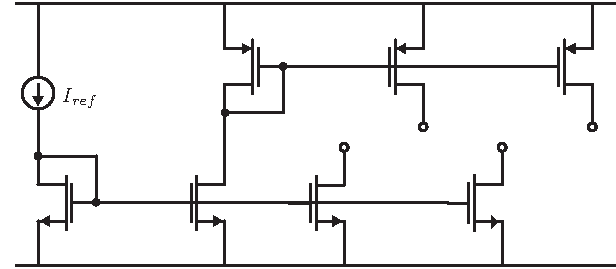
\includegraphics[scale=1.15]{19current_mirror_multioutput.pdf}
\caption{A precision current reference $I_{ref}$ is fed into this circuit and multiple copies are produced, both as current sinks and sources.  Each current can be scaled appropriately as needed.}
\label{fig:current_mirror_multioutput}
\end{figure}
%%%%%%%%%%%%%%%%%%%%%%%%%%%%%%%%%%%%%%%%%%%%%%%%%%%%%%%%%%%%%%%%%%%%%%%%%%%%%%%%%%%%%%%%
%%%%%%%%%%%%%%%%%%%%%%%%%%%%%%%%%%%%%%%%%%%%%%%%%%%%%%%%%%%%%%%%%%%%%%%%%%%%%%%%%%%%%%%%
%                                   SECTION 13.5                                       %
%%%%%%%%%%%%%%%%%%%%%%%%%%%%%%%%%%%%%%%%%%%%%%%%%%%%%%%%%%%%%%%%%%%%%%%%%%%%%%%%%%%%%%%%
%%%%%%%%%%%%%%%%%%%%%%%%%%%%%%%%%%%%%%%%%%%%%%%%%%%%%%%%%%%%%%%%%%%%%%%%%%%%%%%%%%%%%%%%
\section{Current Sources and Sinks}
Technically, up to this point we have really been talking about a \textbf{current "sink"}\index{Current sink} since the NMOS transistors can only sink current to ground.  What if we need a \textbf{current "source"}\index{Current source}?  The \textbf{PMOS mirror}\index{Amplifier!PMOS mirror}, shown in \emph{Fig.~\ref{fig:mirror_pmos}}, is exactly the dual of the \textbf{NMOS mirror}, and it simply mirrors a current that is a "source" from the supply.  In all other aspects, such as the output impedance and scaling, it is identical to the NMOS mirror.  The cascode NMOS mirror can also be replicated and realized in PMOS form. 
%\begin{figure}[tb]
%\centering
%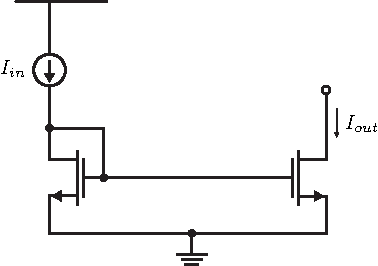
\includegraphics[width=.5\columnwidth]{nmos_source_mirror}
%\caption{nmos source mirror} \label{fig:nmos_source_mirror}
%\end{figure}
%%%%%%%%%%%%%%%%%%%%%%%%%%%%%%%%%%%%%%%%%%%%
%             SUBSECTION 13.5.1            %
%%%%%%%%%%%%%%%%%%%%%%%%%%%%%%%%%%%%%%%%%%%%
\subsection{Generating Multiple Outputs}
One nice observation is that a current mirror can have multiple outputs.  Think of the NMOS diode as a voltage $V_{GS}$ reference.  We can "export" this reference to multiple transistors in parallel, and each will carry a copy of the reference current, appropriately scaled if desired.  The same reference can then be fed into a PMOS mirror, and the PMOS mirror can likewise produce multiple copies of the current.  These currents can be mirrored to various circuit building blocks as required.  As illustrated in \emph{Fig.~\ref{fig:current_mirror_multioutput}}, take note that only a single precision $I_{ref}$ is needed to generate dozens or even hundreds of copies.  In \emph{Sec.~\ref{sec:Ireference}} we will discuss one simple way to generate this reference that is independent of the supply voltage.
\newpage
%%%%%%%%%%%%%%%%%%%%%%%%%%%%%%%%%%%%%%%%%%%%%%%%%%%%%%%%%%%%%%%%%%%%%%%%%%%%%%%%%%%%%%%%
%%%%%%%%%%%%%%%%%%%%%%%%%%%%%%%%%%%%%%%%%%%%%%%%%%%%%%%%%%%%%%%%%%%%%%%%%%%%%%%%%%%%%%%%
%                                   SECTION 13.6                                       %
%%%%%%%%%%%%%%%%%%%%%%%%%%%%%%%%%%%%%%%%%%%%%%%%%%%%%%%%%%%%%%%%%%%%%%%%%%%%%%%%%%%%%%%%
%%%%%%%%%%%%%%%%%%%%%%%%%%%%%%%%%%%%%%%%%%%%%%%%%%%%%%%%%%%%%%%%%%%%%%%%%%%%%%%%%%%%%%%%
\section{Example:  Source-Follower with Real Current Source}
In this example, we will \textbf{bias}\index{Amplifier!biasing!common drain using a current mirror} a source-follower (common drain amplifier) using a current mirror, as shown in \emph{Fig.~\ref{fig:cd_amp_dc}}.  The gate bias voltage $V_{bias,Q}$ needs to be large enough so that the resulting $V_{DS}$ on the drain of the mirror does not "squash" the transistor into the triode region.  Other than that there is a lot of flexibility, making this circuit very useful.  In multi-stage amplifiers, the DC bias of the previous stage driving this circuit just needs to be large enough, but the exact value does not matter.
\vspace{0.5cm}
%%%%%%%%%%%%%%%%%%%%%%%%%%%%%%%%%%%%%%%%%%%%
%                 FIGURE                   %
%%%%%%%%%%%%%%%%%%%%%%%%%%%%%%%%%%%%%%%%%%%%
\begin{figure}[H]
\centering
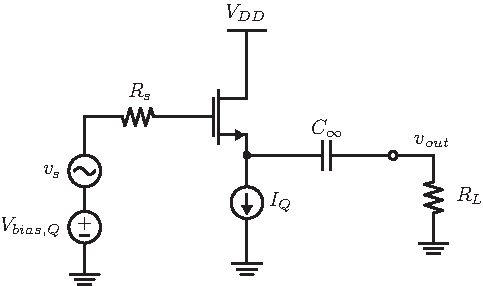
\includegraphics[scale=1.35]{cd_amp_dc}\\
(a)\\[1cm]
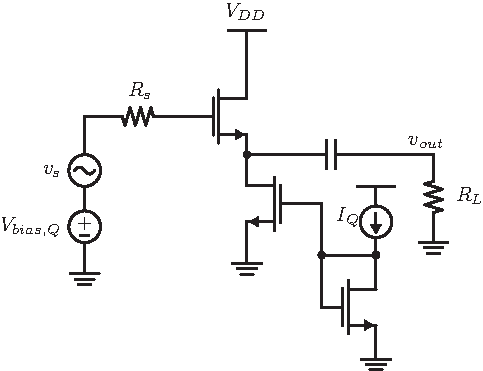
\includegraphics[scale=1.35]{cd_amp_dc_mirror}\\
((b)\\
\caption{(a) A MOS source-follower amplifier using an ideal current source is replaced with (b) a current mirror biased amplifier.}
\label{fig:cd_amp_dc}
\end{figure}
%%%%%%%%%%%%%%%%%%%%%%%%%%%%%%%%%%%%%%%%%%%%
\newpage
%%%%%%%%%%%%%%%%%%%%%%%%%%%%%%%%%%%%%%%%%%%%
%                 FIGURE                   %
%%%%%%%%%%%%%%%%%%%%%%%%%%%%%%%%%%%%%%%%%%%%
\begin{figure}[t]
\centering
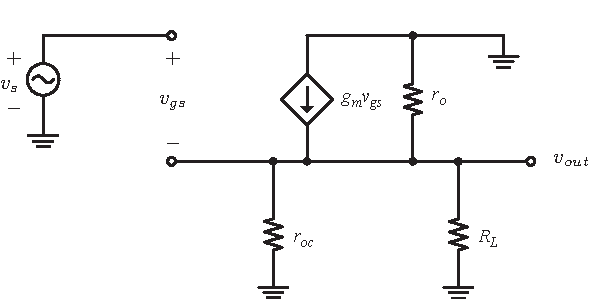
\includegraphics[scale=1.25]{cd_amp_ss_av.pdf}
\caption{Small-signal model of a source-follower biased with a current mirror, modeled as $r_{oc}$.} \label{fig:cd_amp_ss_av.pdf}
\end{figure}
%%%%%%%%%%%%%%%%%%%%%%%%%%%%%%%%%%%%%%%%%%%%
%%%%%%%%%%%%%%%%%%%%%%%%%%%%%%%%%%%%%%%%%%%%
%             SUBSECTION 13.6.1            %
%%%%%%%%%%%%%%%%%%%%%%%%%%%%%%%%%%%%%%%%%%%%
\subsection{Common Drain AC Schematic}
The analysis of the AC response using a small-signal model is easily accomplished by simply noting that the current source can be modeled with an effective output resistance $r_{oc}$, as shown in \emph{Fig.~\ref{fig:cd_amp_ss_av.pdf}}.
%\begin{figure}[tb]
%\centering
%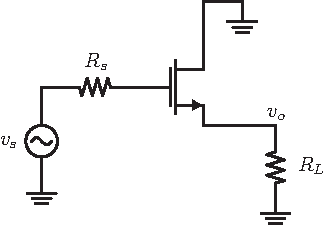
\includegraphics[width=.5\columnwidth]{cd_amp_ac}
%\caption{cd amp ac} \label{fig:cd_amp_ac}
%\end{figure}
%%%%%%%%%%%%%%%%%%%%%%%%%%%%%%%%%%%%%%%%%%%%
%             SUBSECTION 13.6.2            %
%%%%%%%%%%%%%%%%%%%%%%%%%%%%%%%%%%%%%%%%%%%%
\subsection{CD Voltage Gain With Real Current Source}
For an ideal current source, we have:
    \begin{equation}
        \frac{v_{out}}{R_L \parallel r_o} = g_m\,v_{gs} = g_m(v_s - v_{out})
    \end{equation}
With the NMOS current mirror biasing scheme, all we have to do is add the effect of $r_{oc}$: 
    \begin{equation}
        \frac{v_{out}}{R_L \parallel r_o \parallel r_{oc}} = g_m\,v_{gs} = g_m(v_s - v_{out})
    \end{equation}
Let's define an effective load resistance:
    \begin{equation}
        R_{L_{eff}} =  R_L \parallel r_o \parallel r_{oc}
    \end{equation}
From KCL at the output we have:
    \begin{align}
        v_{out} &= g_m\,R_{L_{eff}}\,(v_s - v_{out})\\
        &= g_m\,R_{L_{eff}}\,v_s - g_m\,R_{L_{eff}}\,v_{out}
    \end{align}
Rearranging, and factoring $v_{out}$:
    \begin{equation}
        v_{out} \left(1 + g_m\,R_{L_{eff}}\right) = g_m\,R_{L_{eff}}\,v_s
    \end{equation}
Thus, the voltage gain is given by:
    \begin{align}
        \Aboxed{G_v &= \frac{v_{out}}{v_s} = \frac{g_m\,R_{L_{eff}}}{1 + g_m\,R_{L_{eff}}}}
        &\textit{CD voltage gain with current source}
    \end{align}
\newpage
%%%%%%%%%%%%%%%%%%%%%%%%%%%%%%%%%%%%%%%%%%%%
%                 FIGURE                   %
%%%%%%%%%%%%%%%%%%%%%%%%%%%%%%%%%%%%%%%%%%%%
\begin{figure}[t]
\centering
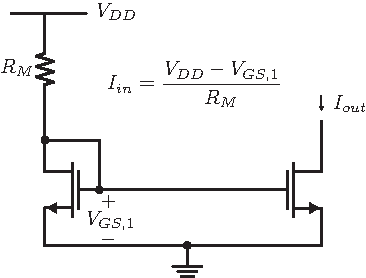
\includegraphics[scale=1.5]{mirror_resistor.pdf}
\caption{A reference current generator using a resistor.  While it's very simple and convenient, it's supply and temperature dependent.}
\label{fig:iref_gen_rs}
\end{figure}
%%%%%%%%%%%%%%%%%%%%%%%%%%%%%%%%%%%%%%%%%%%%%%%%%%%%%%%%%%%%%%%%%%%%%%%%%%%%%%%%%%%%%%%%
%%%%%%%%%%%%%%%%%%%%%%%%%%%%%%%%%%%%%%%%%%%%%%%%%%%%%%%%%%%%%%%%%%%%%%%%%%%%%%%%%%%%%%%%
%                                   SECTION 13.7                                       %
%%%%%%%%%%%%%%%%%%%%%%%%%%%%%%%%%%%%%%%%%%%%%%%%%%%%%%%%%%%%%%%%%%%%%%%%%%%%%%%%%%%%%%%%
%%%%%%%%%%%%%%%%%%%%%%%%%%%%%%%%%%%%%%%%%%%%%%%%%%%%%%%%%%%%%%%%%%%%%%%%%%%%%%%%%%%%%%%%
\section{Generation of Current References}
\label{sec:Ireference}
Up until now we have been ignoring the elephant in the room, which is how to generate the $I_{ref}$ or input current into the mirror.  The simplest way is to simply use a resistor, as shown in \emph{Fig.~\ref{fig:iref_gen_rs}}.  This solution is simple, but it depends on several parameters that may vary.

Some of these parameters include the supply voltage, the transistor threshold voltage $V_T$, and many other parameters such as temperature.  The reference current generated by using a resistor is found with:
    \begin{equation}
        I_{ref} = \frac{V_{DD} - V_{GS,1}}{R_M}  
    \end{equation}
Note that $V_{GS,1}$ is a weak function of $I_{ref}$:
    \begin{equation}
        V_{GS,1} = V_T + \sqrt{\frac{2 I_{ref}}{\mu C_{ox} \frac{W}{L}}}
    \end{equation}
We can solve the above equation to obtain $I_{ref}$.
%%%%%%%%%%%%%%%%%%%%%%%%%%%%%%%%%%%%%%%%%%%%
%                 FIGURE                   %
%%%%%%%%%%%%%%%%%%%%%%%%%%%%%%%%%%%%%%%%%%%%
\begin{figure}[t]
\centering
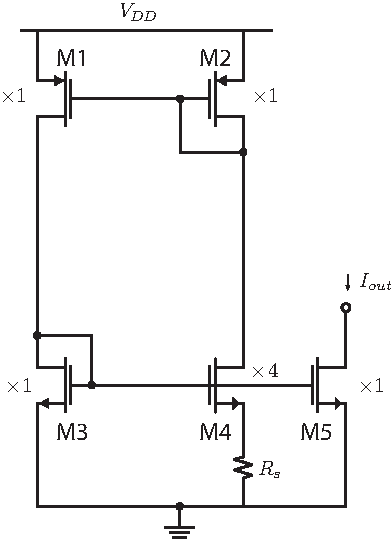
\includegraphics[scale=1.35]{constant_gm_bias.pdf}
\caption{A reference current generator with an output current that produces a constant $g_m = 1/R_s$, independent of supply voltage and temperature.}
\label{fig:constant_gm_ref}
\end{figure}
%%%%%%%%%%%%%%%%%%%%%%%%%%%%%%%%%%%%%%%%%%%%
%             SUBSECTION 13.7.1            %
%%%%%%%%%%%%%%%%%%%%%%%%%%%%%%%%%%%%%%%%%%%%
\subsection{Constant \texorpdfstring{$G_m$}{Transconductance} Reference Current}
What we desire is a supply and temperature independent reference current.  To the greatest extent possible, we want a current that does not depend on transistor parameters, which vary over process and temperature.  There are many clever circuits, such as band gap references, that generate precision temperature independent voltages.  However, in order to generate a current we need a resistor.  Furthermore, unless it is an external precision resistor, there will be variations.  Calibration procedures are needed to tune the currents, a subject beyond the scope of this book.

Here we will not delve into the details of various circuits to build references.  Instead we will present a very useful example, which is the constant-$g_m$ reference generator, shown in \emph{Fig.~\ref{fig:constant_gm_ref}}.  This example is a particularly good one because it is simple, and it builds on the principles we have already discussed in this chapter.

With reference to \emph{Fig.~\ref{fig:constant_gm_ref}}, notice that the PMOS mirror on top enforces current equality between the two branches, as the devices have the same dimensions.  In other words, the currents $I_{D_3}$ and $I_{D_4}$ must be equal.  On the other hand, the bottom current sources are not sized the same, and transistor $M3$ is sized to be exactly $1/4$ smaller than $M4$.  The voltage across the resistor $R_s$ is given by:
    \begin{equation}
        V_{R_S} = \Delta V_{GS} = V_{GS_3} - V_{GS_4}
    \end{equation}
We can express each $V_{GS}$ as a threshold voltage plus an overdrive voltage:
    \begin{equation}
        V_{GS_4} = V_T + \sqrt{\frac{2\,I_{D_4}}{\mu\,C_{ox} \left(\frac{W}{L}\right)_4}} = V_T + V_{OD_4}
    \end{equation}
For device $M3$, it carries the same current and has a 4 times smaller width:
    \begin{equation}
        V_{GS_3} = V_T + \sqrt{\frac{2\,I_{D_4}}{\mu\,C_{ox} \left(\frac{W}{4L}\right)_4}} = V_T + 2V_{OD_4}
    \end{equation}
With this observation, the output current of $M4$ is simply given by:
    \begin{equation}
        I_{D_4} = \frac{\Delta V_{GS}}{R_S} = \frac{V_{OD_4}}{R_S}
        \label{eq:gm_constant}
    \end{equation}
Substitution of the overdrive voltage leads to the output current:
    \begin{equation}
        I_{D_4} = \frac{V_{OD_4}}{R_S} = \frac{1}{R_S} \sqrt{\frac{2\,I_{D_4}}{\mu C_{ox} \left(\frac{W}{L}\right)_4}}
        \label{eq:reference_current_sub}
    \end{equation}
Or, by squaring both sides of \emph{Eq.~\ref{eq:reference_current_sub}}, and dividing both sides by $I_{D_4}$:
    \begin{equation}
        I_{D4} = \frac{1}{{R_S}^2} \frac{2}{\mu C_{ox} \left(\frac{W}{L}\right)_4}
    \end{equation}	
Notice that the current $I_{D_4}$ does not depend on the supply voltage or the device threshold, so it can be used as a reference current.  If we mirror the current of $M3$ to another transistor of equal size, it will satisfy \emph{Eq.~\ref{eq:gm_constant}}.  This is a nice circuit, because the ratio of current to overdrive voltage, which is related to the transconductance, tracks $R_S$:
    \begin{equation}
        g_{m_5} = \frac{2\,I_{D_5}}{V_{OD_5}} = \frac{\cancel{2}\,I_{D4}}{\cancel{2}\,V_{OD_4}} = \frac{1}{R_S}
    \end{equation}
For this reason, this circuit is known as a \textbf{constant transconductance reference}\index{Amplifier!constant transconductance reference}, because all transistors biased with this current will have a $g_m$ that is constant and independent of process and temperature.
%%%%%%%%%%%%%%%%%%%%%%%%%%%%%%%%%%%%%%%%%%%%
% \newpage
% %%%%%%%%%%%%%%%%%%%%%%%%%%%%%%%%%%%%%%%%%%%%%%%%%%%%%%%%%%%%%%%%%%%%%%%%%%%%%%%%%%%%%%%%
% %%%%%%%%%%%%%%%%%%%%%%%%%%%%%%%%%%%%%%%%%%%%%%%%%%%%%%%%%%%%%%%%%%%%%%%%%%%%%%%%%%%%%%%%
% %                                 SECTION 13.8                                         %
% %%%%%%%%%%%%%%%%%%%%%%%%%%%%%%%%%%%%%%%%%%%%%%%%%%%%%%%%%%%%%%%%%%%%%%%%%%%%%%%%%%%%%%%%
% %%%%%%%%%%%%%%%%%%%%%%%%%%%%%%%%%%%%%%%%%%%%%%%%%%%%%%%%%%%%%%%%%%%%%%%%%%%%%%%%%%%%%%%%
% \section{Chapter Summary}
% In this chapter we ...
